%% LyX 2.0.8.1 created this file.  For more info, see http://www.lyx.org/.
%% Do not edit unless you really know what you are doing.
\documentclass[american,english]{report}
\usepackage{lmodern}
\renewcommand{\sfdefault}{lmss}
\renewcommand{\ttdefault}{lmtt}
\usepackage[T1]{fontenc}
\usepackage[latin9]{inputenc}
\usepackage{geometry}
\geometry{verbose,tmargin=3cm,bmargin=3cm,lmargin=4cm,rmargin=4cm}
\setcounter{secnumdepth}{3}
\setcounter{tocdepth}{3}
\usepackage{array}
\usepackage{float}
\usepackage{url}
\usepackage{amsmath}
\usepackage{amssymb}
\usepackage{graphicx}
%\usepackage{minted}
\usepackage[]{mcode}

\makeatletter

%%%%%%%%%%%%%%%%%%%%%%%%%%%%%% LyX specific LaTeX commands.
%% Because html converters don't know tabularnewline
\providecommand{\tabularnewline}{\\}

%%%%%%%%%%%%%%%%%%%%%%%%%%%%%% User specified LaTeX commands.
\usepackage{microtype}
\usepackage{listings}
\usepackage[compact]{titlesec}  
\titlespacing{\section}{0pt}{5pt}{0pt}
\titlespacing{\subsection}{0pt}{3pt}{0pt}
\titlespacing{\subsubsection}{0pt}{2pt}{0pt}
%\titleclass{\chapter}{straight}
\titleformat{\chapter}[hang] {\LARGE\bf}{\LARGE\thechapter}{1ex}{}[]
\titlespacing{\chapter}{0pt}{10pt}{5pt}

\usepackage{fancyhdr}
\fancyhead{} \fancyfoot{}
\fancyhead[LO,LE]{{\bf MSE-639}}
\fancyhead[RO,RE]{Prof. Michele Ceriotti }
\fancyfoot[LO,LE]{Statistical Methods in Atomistic Computer Simulations}
\fancyfoot[RO,RE]{ \thepage}

\usepackage{chngcntr}
\counterwithout{figure}{chapter}

\makeatother

\usepackage{babel}
\begin{document}
\newcommand{\D}{\ensuremath{\mathrm{d}}}

\newcommand{\I}{\ensuremath{\mathrm{i}}}

\setlength{\parskip}{0.3ex}
\setlength{\parindent}{2mm}
\let\olditem\item \renewcommand{\item}{\setlength{\parskip}{0.1ex}\setlength{\itemsep}{0.1ex}\olditem}

{\centering \Large \bfseries Statistical methods in atomistic computer
simulations\\\vspace{2mm}}

{\centering \emph{Prof. Michele Ceriotti, michele.ceriotti@epfl.ch\\ Piero Gasparotto, piero.gasparotto@epfl.ch}\\\vspace{5mm}}

{\centering Hands-on exercises on a Lennard-Jones 38 cluster \\\vspace{15mm}}\thispagestyle{empty}

The system that will be examined is a clusters of 38 atoms interacting
with a simple Lennard-Jones (LJ) potential:
\[
U\left(r\right)=4\epsilon\left[\left(\frac{\sigma}{r}\right)^{12}-\left(\frac{\sigma}{r}\right)^{6}\right]
\]
where $\epsilon$ is the well depth and $2^{\frac{1}{6}}\sigma$ is
the equilibrium separation for a diatomic molecule. This potential
describes dipole fluctuation attractive interactions that decay as
$r^{-6}$, and a somewhat arbitrary $r^{-12}$ repulsive wall at short
inter-atomic separations, that models the Pauli repulsion between
electron clouds. The Lennard-Jones potential is a good model for the
interaction between noble gases atoms, but here we will use it just
as an inexpensive model of an isotropic pair-wise interaction between
atoms. In all the exercises reduced units will be used, that correspond
to measuring energies in units of $\epsilon$, distances
in units of $\sigma$, time in units of $t^{*}=\left(\frac{\epsilon}{m\sigma^{2}}\right)$,
and temperature in units of $T^{*}=\left(\frac{k_{B}}{\epsilon}\right)$.
In practice this amounts at setting to one most constants: in principle
all results can be scaled to the physical values for a particular
system by setting the appropriate mass, well depth and equilibrium
distance. 

A LJ cluster provides a particularly useful model system since for
small LJ clusters a complete enumeration of the minima and transition
states allows a detailed view of the potential energy landscape~\cite{wale03book}.
In particular the LJ$_{38}$ , the cluster which we study here, has
a double-funnel landscape: the global minimum is a face-centered-cubic
(fcc) truncated octahedron (Fig. \ref{fig:minimalj38}(a)) and the
second lowest energy minimum is an incomplete Mackay icosahedron (Fig.
1(b)).

\begin{center}
\begin{figure}[H]
\caption{\selectlanguage{american}%
\label{fig:minimalj38}\foreignlanguage{english}{(a) The LJ$_{38}$
global minimum, an fcc truncated octahedron. (b) and (c) Second lowest
energy minimum of LJ$_{38}$. Figure adapted from \cite{doye_double-funnel_1999}.}\selectlanguage{english}%
}


\centering{}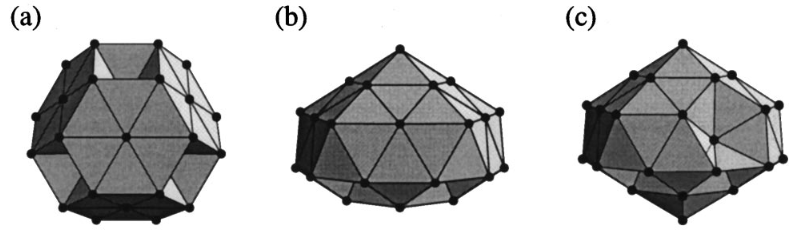
\includegraphics[width=0.7\textwidth]{figures/minimalj38}
\end{figure}

\par\end{center}

There is thus a solid--solid transition at moderate temperatures and
a subsequent solid--liquid transition at higher temperatures. The
solid--solid transition occurs because the energy landscape in the
high-temperature phase is flatter, resulting in a larger entropic
contribution to the free energy of this structure, and to its stabilization
at moderate temperatures relative to the \emph{fcc} minimum~\cite{ceriotti_demonstrating_2013}.
Figure~\ref{fig:lj38michele} shows a few selected configurations
for this system, together with the free energy computed close to the
solid-liquid transition temperature. The stability of different configurations
depends dramatically on the simulation temperature, and the time scales
for transitions is long, but accessible to direct simulation thanks
to the small size and inexpensive potential. This makes LJ$_{38}$
an ideal example to show the strength and pitfalls of different sampling
techniques in atomistic simulations. 

\begin{center}
\begin{figure}[H]
\caption{\selectlanguage{american}%
\label{fig:lj38michele}\foreignlanguage{english}{A number of representative
configurations of the LJ$_{38}$ cluster are projected together with
the free energy surface computed at 0.18$T^{*}$. Figure adapted from
\cite{ceriotti_demonstrating_2013}}\selectlanguage{english}%
}


\centering{}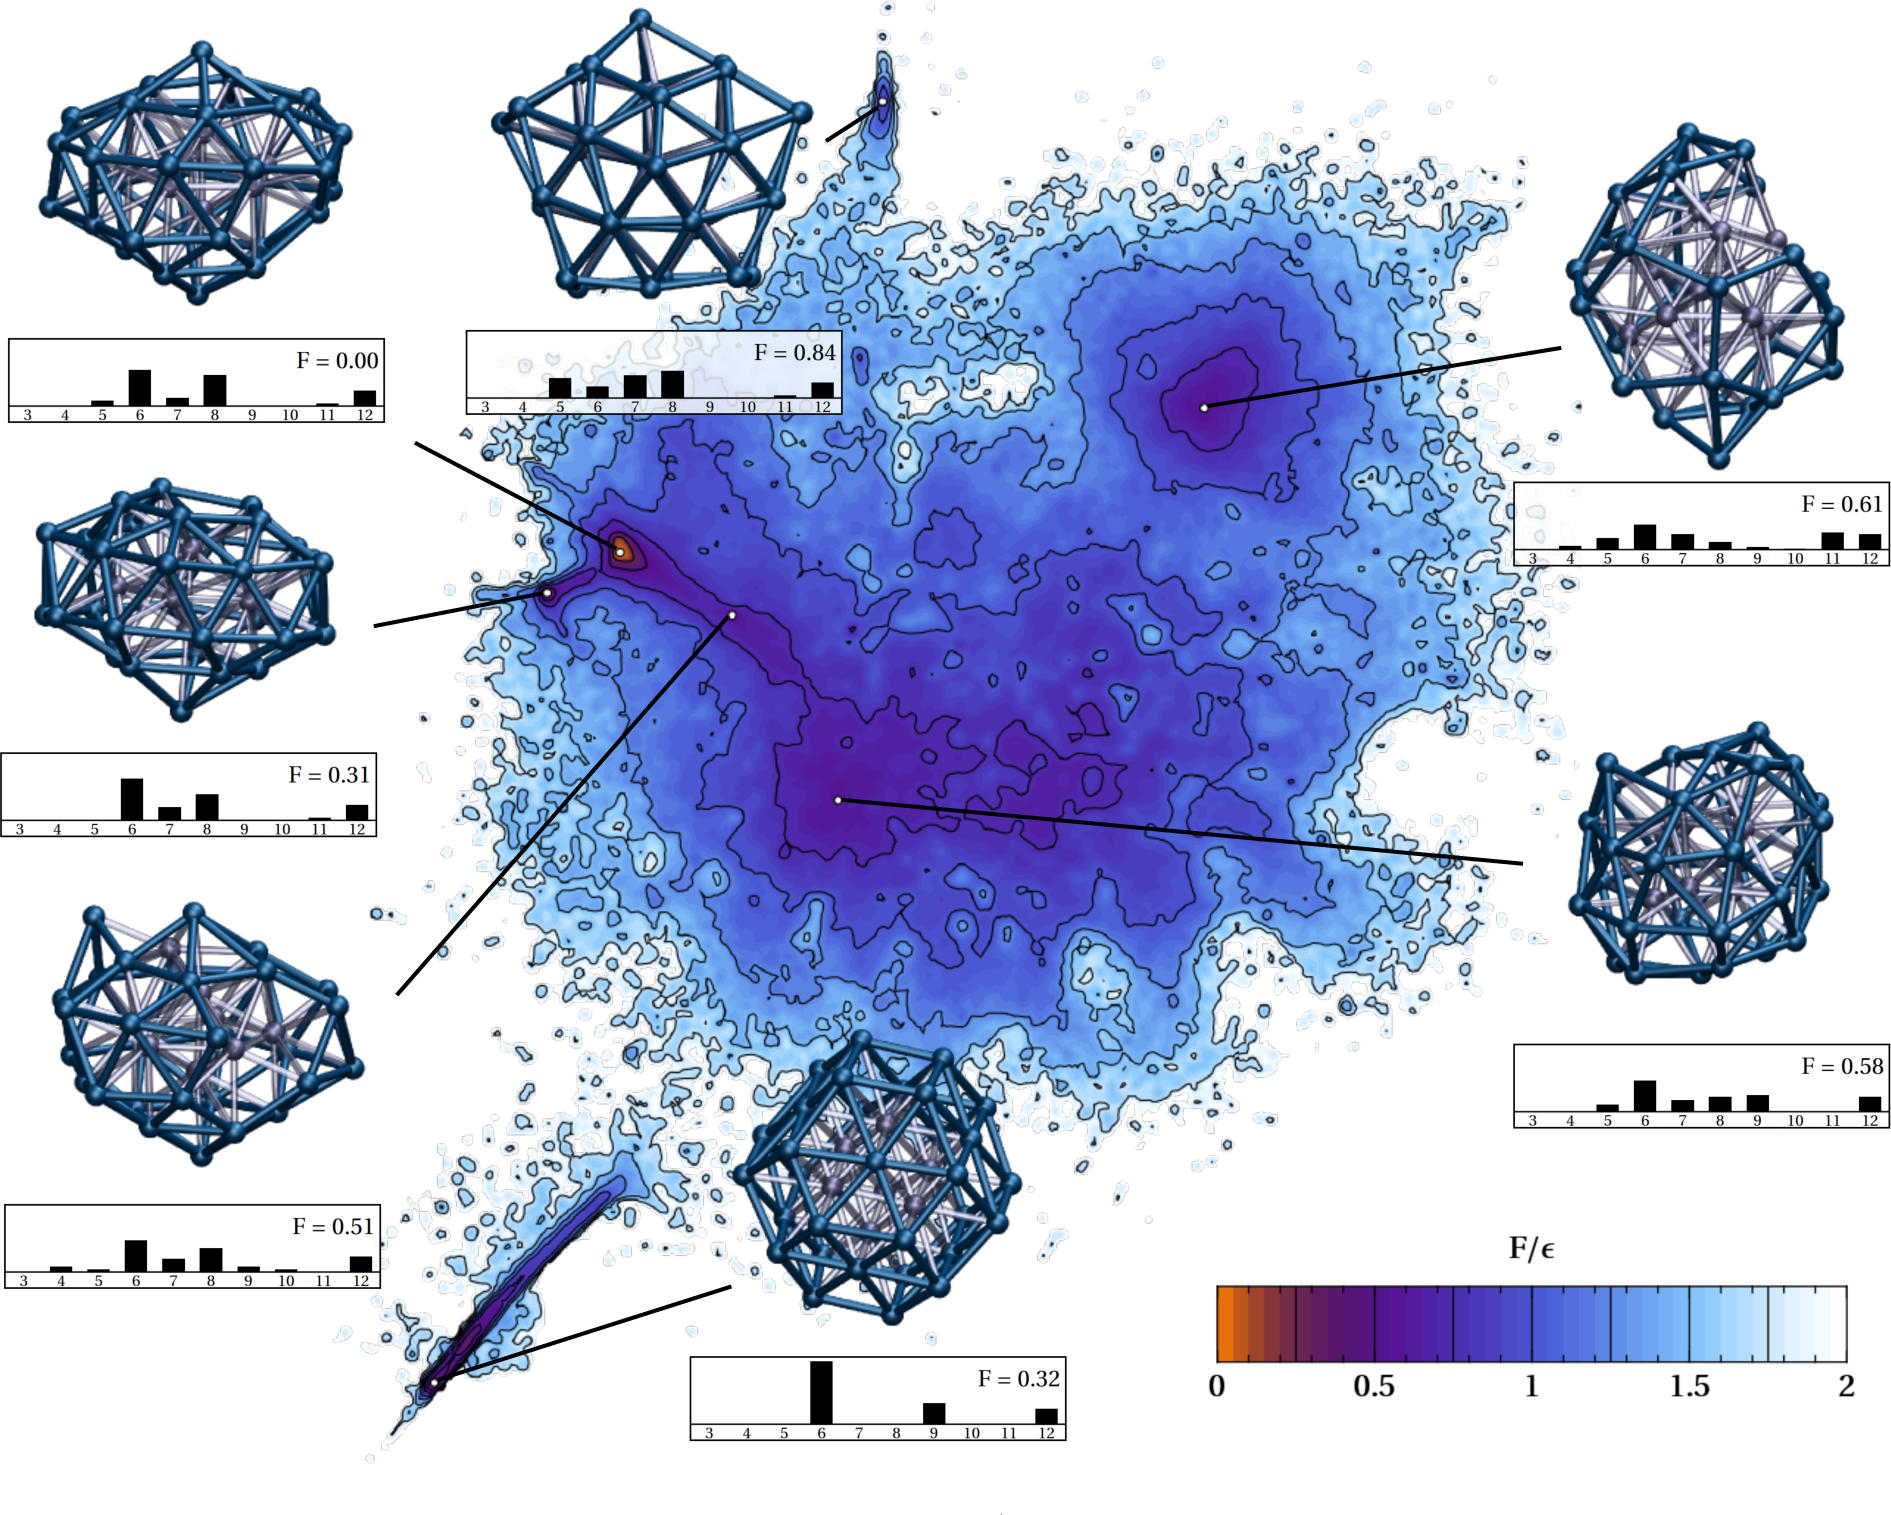
\includegraphics[width=0.9\textwidth]{figures/lj38michele}
\end{figure}

\par\end{center}


\section*{General remarks}

These exercises are structured as a hands-on tutorial, in which you
are given simple, rudimentary programs that (should) already work.
You are encouraged to look at the source code to understand how things
work, and you are more than welcome if you want to clean up the code,
include better comments or more explanatory error messages.

You should be able to finish most of the exercises in two hours. Please
keep your results in order, as you will be asked to put them together
in a short report in which you explain what you learned from each
part of the tutorial, and since at times you will have to compare
results obtained from different exercises. 

Always \textbf{change the random number seed} in the example input files before
you run: in this way each one will have statistically independent
results, and it will be possible to combine the results of different
groups to get more converged statistics. It is expected for you to
be familiar with running programs from a UNIX shell. If this is not
the case, it is highly recommended that you follow one of the many
excellent tutorials that can be found on-line before you start.


\section*{Utility programs}

The programs used to \emph{run} simulations have been developed specifically
for this course, and are distributed as a package together with these
notes. However, a few utilities will be used to post-process the simulation
output -- for instance to compute histograms and autocorrelation functions.
These should be downloaded from their \texttt{git} repositories, and
then compiled:

\begin{lstlisting}[language=matlabfloz]
$ git clone https://github.com/epfl-cosmo/toolbox.git
$ cd toolbox/src
$ make
$ cd ..
\end{lstlisting}You may need to create a \texttt{make.in} file based on \texttt{make.in.example},
and to install lapack and fftw3 to have access to all the features
of this set of utilities. On a Debian/Ubuntu system, you should be
able to do so by running 

\begin{lstlisting}[language=matlabfloz]
$ cp make.example.in make.in
$ sudo apt-get install libfftw3-dev liblapack-dev
\end{lstlisting}

For the last exercise, you will also need the \texttt{sketchmap }suite
of dimensionality reduction programs. You should be able to get it
from the repository \\

 \texttt{https://github.com/epfl-cosmo/sketchmap.git}\\

Lastly, in some steps you will be asked to visualize your structure trajectories using the \texttt{vmd} command.
In order to use it, you'll have to install it from its webpage  \\

 \texttt{http://www.ks.uiuc.edu/Development/Download/download.cgi?PackageName=VMD}\\


\chapter{Monte Carlo}

\lstset{language=bash} 

This exercise is meant to be a simple introduction to Metropolis Monte
Carlo (MC), and a way to get familiar with the LJ$_{38}$ system and
with the programs we will use to post-process the simulation data.
You will find the source code in the \texttt{src/ }directory, that
contains

\begin{center}
\begin{minipage}[t]{0.8\textwidth}%
\begin{tabular*}{0.6\paperwidth}{@{\extracolsep{\fill}}lp{0.7\textwidth}}
\texttt{mcnvt.f90} & The main file, containing the initialization of the system and the
Metropolis MC algorithm\tabularnewline
\texttt{routines.f90} & The module containing the principal functions and subroutines used
in the \texttt{mcnvt.f90} file, such as the calculation of the energy,
the i/o routines, ...\tabularnewline
\texttt{random.f90} & Routines to sample a uniform and Gaussian random numbers\tabularnewline
\texttt{Makefile} & The file containing the compilation parameters\tabularnewline
\end{tabular*}%
\end{minipage}
\par\end{center}

First, try to familiarize yourself with the source, which is heavily
commented and should allow you to easily follow the algorithms. Compilation
is straightforward:\begin{lstlisting}[language=matlabfloz]
$ pwd
~/exercises/ex1
$ cd src
$ make
$ cd ..
\end{lstlisting}

This will generate a binary file called \texttt{mcnvt}, that you will
use to run the exercises. The input file for \texttt{mcnvt} contains
the following options:

\begin{center}
\begin{minipage}[t]{0.8\textwidth}%
\begin{tabular*}{0.6\paperwidth}{@{\extracolsep{\fill}}lp{0.7\textwidth}}
\texttt{\&inp } & \tabularnewline
\texttt{seed = 1357} & Initial seed for the random number generator\tabularnewline
\texttt{temp = 0.23} & Target temperature\tabularnewline
\texttt{dataxyz = 'lj38.xyz'} & Starting configuration (xyz format)\tabularnewline
\texttt{nstep = 10000000} & Number of steps to be performed\tabularnewline
\texttt{stridetrj = 10000} & Output stride for the trajectory\tabularnewline
\texttt{stridelog = 100} & Output stride for the simulation logs\tabularnewline
\texttt{mcstep = 0.001} & Variance of the Gaussian random numbers used to generate trial configurations\tabularnewline
\texttt{outputf = 'out.xyz'} & Output trajectory file\tabularnewline
\texttt{\&end} & \tabularnewline
\end{tabular*}%
\end{minipage}
\par\end{center}


\section{MC equilibration}

In this exercise we will study the equilibration of the system in
the \emph{NVT }ensemble. The proposed target temperature is $0.23\, T^{*}$.
The starting initial configuration contained in the file \texttt{lj38.xyz}
is the \emph{fcc} truncated octahedron relaxed to $0\, T^{*}$.

Launch the program with the following command:

\begin{lstlisting}[language=matlabfloz]
$ ../src/mcnvt input > log &
\end{lstlisting}This will output the statistics in the file \texttt{log }and will
run the calculation in background so you can monitor the equilibration
of the system using \texttt{gnuplot}. For instance, to plot the potential
energy as a function of the number of MC steps:

\begin{lstlisting}[language=matlabfloz]
$ gnuplot
 gnuplot> p 'log' u 1:2 w l 
(alternatively: gnuplot> plot 'log' using 1:2 with line)
\end{lstlisting}

\begin{itemize}
\item Observe how the potential energy converges to the equilibrium value
\item Look at the trajectory file using 
\begin{lstlisting}[language=matlabfloz]
$ vmd out-023.xyz
\end{lstlisting}
and experiment with the visualization options of \texttt{vmd} (particularly in the menu graphics -> representations). 
\item Check how the equilibration varies when changing the input parameters,
such as \texttt{mcstep} and the target temperature
\item The transient that is observed at the beginning of the equilibration
is related to the sampling efficiency (because of the connection between
relaxation to equilibrium and fluctuations in the equilibrium ensemble).
The sampling efficiency can be estimated by computing the autocorrelation
time.

\begin{itemize}
\item use the \texttt{autocorr} tool to compute the autocorrelation function
from one of the logs
\begin{lstlisting}[language=matlabfloz]
$ tail -n +10000 log | awk '!/#/{print $2}' 
| autocorr -maxlag 10000 -timestep 100 > acf
\end{lstlisting}
The \texttt{-maxlag} option specifies the time window in which to
calculate the autocorrelation function, while the \texttt{-timestep}
flag is used to set the unit of time based on the stride and timestep
used for the trajectory, so that the time scale output from \texttt{autocorr}
corresponds to the correct simulation time. Note that we use \texttt{tail}
to remove the first part of the trajectory (which consists of the
equilibration, so the number of dropped lines should be adjusted depending
on the length of the transient!), and \texttt{awk} to pick the column
that corresponds to the potential energy. 
\item the program returns extensive statistical data about the trajectory.
The header contains the average and standard deviation of the data
set, the autocorrelation time and an estimate of the error in the
mean obtained from the variance of the data, the autocorrelation time
and the the length of the trajectory.\begin{lstlisting}[language=matlabfloz]
$ head acf 
...
#  computed with time unit:    1.0000000e+02     # 
#  mean:      -1.5525889e+02 +- 2.9949957e-01    # 
#  sigma:     2.4443721e+00                      # 
#  a.c. time: 4.5166879e+05                      #
...
\end{lstlisting} Then, a series of time-dependent diagnostics follows, where the first
line indicate the time and the second column the value of the autocorrelation
function -- you can ignore the other columns. Plot the autocorrelation
function using gnuplot, and observe how the decay to zero varies with
the MC step.
\item compute the autocorrelation function of trajectories of different
length. See how the autocorrelation function requires very long trajectories
to reach convergence, and how the tail of the function tends to be
noisy. Since \texttt{autocorr} evaluates the autocorrelation time
as the integral up to the maximum time lag, the \texttt{-maxlag} option
should be set to be long enough for the function to converge to zero,
but not much longer, to avoid picking noise from the tail, which would
affect the estimate of the correlation time. 
\end{itemize}
\end{itemize}

\section{Optimization of the MC step}

Since the autocorrelation time directly relates to the statistical
efficiency of sampling, it is crucial to choose a MC step that minimizes
the autocorrelation time. Here we will perform a systematic study
using many different values in order to understand the trend of $\tau_{A}$
as a function of the the \texttt{mcstep}. We will also see how the
optimal correlation time compares with the acceptance ratio $\alpha=\frac{\text{\text{accepeted moves}}}{\text{total moves}}$.
\begin{itemize}
\item Perform a series of separate runs changing the value of the \texttt{mcstep
}parameter, and compute for each of the runs the autocorrelation time.
Start with the examples provided. Make sure that the simulation is
long enough to converge the autocorrelation function, and that the
maximum lag is not much longer than the autocorrelation time itself.
Also, keep track of the acceptance ratio, which is printed out at
the end of each run as a comment in the log file: \begin{lstlisting}[language=matlabfloz]
$ tail -n 6 log-0.05
##  
## Total moves:        50000  
## Accepteed moves:        11277  
##  
## Ratio:   0.22553999999999999       
##
\end{lstlisting}
\item Write down in a text file the autocorrelation time and the acceptance
ratio as a function of the \texttt{mcstep}. You can then use \texttt{gnuplot}
to generate a plot and store it in an image that you can use when
you write your report. To export graphs produced by \texttt{gnuplot,
}you can just specify a terminal, which also determines the format
of output file. \texttt{gnuplot} supports terminals for various formats
including png, jpg, gif and postscript. For instance, \begin{lstlisting}[language=matlabfloz]
gnuplot> set terminal png size 400,300 enhanced font "Sans,20"
gnuplot> set output "mcstep.png"
\end{lstlisting}In this example we used the png output format, but you can either
use jpg, ps and pdf. The other options used -- size, enhanced, font
-- let you to control the appearance of the exported plot.
\item Which value of \texttt{mcstep} corresponds to the shortest autocorrelation
time? What is the corresponding $\alpha$?
\end{itemize}

\section{Exploiting local moves}

{[}OPTIONAL{]} The program is implemented using the detail balance
Metropolis condition as transition rule : 
\[
\eta<e^{-\beta\left(V^{\text{new}}-V^{\text{new}}\right)}
\]
where $\eta$ is a number between zero and one sampled from a uniform
distribution, while $V^{\text{new}}-V^{\text{new}}$is the energy
difference of the entire system after and before the move. Since we
are using a simple pairwise LJ potential and since we move just one
particle per move, this is a wasteful way to proceed: the potential
is evaluated as a sum of pair terms 
\[
V\left(\left\{ \mathbf{r}_{1},\ldots,\mathbf{r}_{N}\right\} \right)=\frac{1}{2}\sum_{ij}v\left(\left|\mathbf{r}_{i}-\mathbf{r}_{j}\right|\right),
\]
and so moving just one particle leaves most of the pair-wise terms
untouched. In fact, one can show that if the $k$-th particle has
been moved, the difference between the potential before and after
the move is just 
\[
V^{\text{new}}-V^{\text{old}}=\sum_{i}v\left(\left|\mathbf{r}_{i}-\mathbf{r}_{k}^{\text{new}}\right|\right)-\sum_{i}v\left(\left|\mathbf{r}_{i}-\mathbf{r}_{k}^{\text{old}}\right|\right).
\]
You can try to modify the code to use this trick to reduce the cost
of performing each MC step, and see how the wall-clock execution time
changes.


\chapter{Molecular dynamics.}

This exercise focuses on using Molecular Dynamics (MD) to sample the
constant temperature canonical ensemble. Enclosed is a simple MD program
that will give you the possibility to run simulations in the NVE and
NVT ensemble for a Lennard-Jones cluster. In order to couple the system
with a thermal bath, three thermostat are implemented: Andersen, white-noise
Langevin (WNL) and colored-noise Generalized Langevin Equation (GLE).
All the source code files are provided in the \texttt{src/} directory,
that contains

\begin{center}
\begin{minipage}[t]{0.8\textwidth}%
\begin{tabular*}{0.6\paperwidth}{@{\extracolsep{\fill}}l>{\raggedright}p{0.7\textwidth}}
\texttt{mdcode.f90} & The main file, containing the initialization of the system and the
MD loop\tabularnewline
\texttt{routines.f90} & The module containing the principal subroutines used in the \texttt{mdcode.f90}
file, such as the calculation of energies and forces, i/o routines
and basic thermostats\tabularnewline
\texttt{glecn.f90} & The module containing routines for the colored-noise Langevin thermostat\tabularnewline
\texttt{random.f90} & Routines to sample a random number from a Gaussian distribution with
zero mean.\tabularnewline
\texttt{Makefile} & The file containing the compilation parameters\tabularnewline
\end{tabular*}%
\end{minipage}
\par\end{center}

To compile the program just type \texttt{make} as already seen for
the MC code. This will generate a binary file called \texttt{mdcode}.
The input file is as follows:

\begin{center}
\begin{minipage}[t]{0.8\textwidth}%
\begin{tabular}{l>{\raggedright}p{0.7\textwidth}}
\texttt{\&inp } & \tabularnewline
\texttt{seed = 1357} & Initial seed for the random number generator\tabularnewline
\texttt{temp = 0.20} & Target temperature\tabularnewline
\texttt{dataxyz = 'lj38.xyz'} & Starting configuration\tabularnewline
\texttt{dt = 0.001} & Integration time step\tabularnewline
\texttt{nstep = 20000} & Number of steps to be performed\tabularnewline
\texttt{langevinWNtau = 10} & Relaxation time of the white-noise Langevin thermostat. If set to
0, or if the keyword is not present, this thermostat will not be applied\tabularnewline
\texttt{gleafile = 'gle-A.dat'} & The file containing the drift matrix A required by the colored-noise
Langevin thermostat. If set to an empty string or if the keyword is
not present this thermostat will not be applied\tabularnewline
\texttt{mstep = 1} & Apply the Langevin thermostats in a multiple time step fashion\tabularnewline
\texttt{andersentau = 10} & Relaxation time of the Andersen thermostat If set to 0, or if the
keyword is not present, this thermostat will not be applied\tabularnewline
\texttt{stridetrj = 50000} & Stride outputting the trajectory\tabularnewline
\texttt{stridelog = 1} & Stride outputting the simulation logs\tabularnewline
\texttt{outputf = 'out.xyz'} & Output trajectory file\tabularnewline
\texttt{\&end} & \tabularnewline
\end{tabular}%
\end{minipage}
\par\end{center}

Note that using \texttt{langevinWNtau = 0, gleafile = ''} and \texttt{andersentau
= 0} one can perform constant-energy microcanonical dynamics in the
NVE ensemble.


\section{NVE dynamics and energy conservation. }

In MD, Hamiltonian systems of differential equations are numerically
integrated to evolve the system in time following the prescriptions
of classical, Newtonian dynamics. The integrator implemented in \texttt{mdcode}
is the simple (but effective) velocity-Verlet algorithm. Such a method
does not conserve energy exactly along the trajectory, thus leading
to a discretized trajectory that diverges from the one that would
be obtained by exact integration of the dynamics. However, although
it does not conserve the energy, when using a sufficiently small time
step, the velocity-Verlet integrator maintains the system's total
energy in a narrow band around the true energy and yields remarkably
stable trajectories with essentially no significant energy drift.

A word of caution: while one can achieve near-perfect energy conservation
by reducing the time step, working with an excessively small time
step may result in waste of computer time. A practical compromise
would allow for small energy fluctuations and slow energy drifts,
as a price to pay to work with a reasonably large \texttt{dt}. Concerns
about the conservation of total energy are less serious when using
a thermostat, as it will be discussed below. 

As a first example of molecular dynamics, we will run NVE simulations
starting from a configuration frozen in the \emph{fcc }ground state
structure, and try to melt it as we did with Monte Carlo. Use the
example file\texttt{ }called \texttt{input} in the directory \texttt{pt1/}
.

To run the program:\begin{lstlisting}[language=matlabfloz]
$ ../src/mdcode input > log &
\end{lstlisting}Before starting the exercise take a brief look at the \texttt{log}
file:\begin{lstlisting}[language=matlabfloz]
$ head log
## MD code.   
## Natoms:           38  
## Timestep:   1.00000000000000002E-002  
## Temperature:   0.23000000000000001       
##  
## Step, Temp, Ekin, Epot, Etot, Conserved quantity
 0  0.2397 0.1330 -173.9225 -160.6201 -160.6201
 10 0.8079 4.4842 -165.0655 -160.5812 -160.5812
 20 0.1119 6.2140 -166.8071 -160.5931 -160.5931
\end{lstlisting}
\begin{itemize}
\item Use \texttt{gnuplot} to monitor the potential, kinetic and total energies:
\begin{lstlisting}[language=matlabfloz]
gnuplot> p 'log' u 1:3 w l
gnuplot> p 'log' u 1:4 w l, 'log' u 1:5 w l
\end{lstlisting}
\item Try running with increasing values of the time step. What happens?
Visualize the trajectory using \texttt{vmd}. 

\begin{itemize}
\item What is the highest usable timestep?
\item How do energy fluctuations and drift vary with \texttt{dt}?
\end{itemize}
\end{itemize}

Now, choose the best timestep you found and run a simulation at \texttt{$T{}^{*}$=0.20}
lasting for 3 million steps. Look at the trajectory using \texttt{vmd}.
 Plot the potential energy and compare the results with those from
MC simulation at the same target temperature, starting from the same
configuration. 
\begin{itemize}
\item What can you say about the equilibration and energy trend comparing
the MD plot with the MC one?
\item Compute the average temperature and the average configurational energy.


\begin{lstlisting}[language=matlabfloz]
$ tail -n +5000 log | awk '!/#/{t+=$2;pot+=$4; n++} 
 END{print"T=",t/n;print"Epot=",pot/n}'
\end{lstlisting}


What is the value of $\left\langle T^{*}\right\rangle $? And $\left\langle V\right\rangle $?
Are they comparable with the chosen target temperature and with $\left\langle V\right\rangle $
obtained from the MC simulation?

\end{itemize}

\section{Constant temperature MD }

NVE molecular dynamics does not yield sampling consistent with the
target temperature -- particularly if the simulation is initialized
from a configuration which is not compatible with the ensemble. Three
thermostat are implemented in \texttt{mdcode} to perform ergodic trajectories within the NVT ensemble. Go into the directory \texttt{pt2} and run
a first simulation using the provided example file (do not change
the target temperature). \\ 
You should also run the GLE simulation from (2.4) since the simulation should last for an hour.
\begin{itemize}
\item Plot the total energy (or the configurational energy) and compare
it with the one from the NVE run. What happens switching on the thermostat?
Plot also the conserved quantity (column 6). Is it (approximately)
conserved? See that its fluctuations decrease if you reduce the time
step further.
\item Run a new simulation using as starting configuration the final snapshot
from the previous trajectory:


\begin{lstlisting}[language=matlabfloz]
$ tail -n 40 out.xyz > ljnew.xyz &
\end{lstlisting}


Remember to change the input file setting \texttt{dataxyz = 'ljnew.xyz'.}\begin{lstlisting}[language=matlabfloz]
$ sed "s/lj-oct-ok/ljnew/" input > input.new &
\end{lstlisting}
\begin{itemize}
\item Is the equilibration transient changed? If yes, why?
\end{itemize}
\item Now try to increase a bit \texttt{dt} (let's say \texttt{dt=0.01})
and, again, plot the conserved quantity and the total energy together. 

\begin{itemize}
\item What happens to the conserved quantity increasing \texttt{dt}?
\item Does the mean total energy change significantly (use \texttt{autocorr}
to compute a mean value with errorbars)?
\end{itemize}
\item Compute the autocorrelation function for the potential energy and
plot it. Can you see the multiple time scales at play here? Compute
the autocorrelation time and compare it to the efficiency of Monte
Carlo in terms of energy evaluations needed to obtain an uncorrelated
sample. Is this a fair comparison?
\item {[}OPTIONAL{]} Test the Andersen thermostat and compare the resulting
total energy with the one using the WNL from the previous simulation.
What the difference between the two? How does the Andersen's one look
like?

\begin{itemize}
\item What happens choosing a big relaxation time for the Andersen thermostat?
And a really small one?
\end{itemize}
\end{itemize}

\section{Assessing the sampling efficiency of the WNL thermostat }

The sampling efficiency of a thermostat can be assessed quantitatively
evaluating the autocorrelation times relative to the observables we
are interested in. Since the behavior of the WNL thermostat is controlled
tuning its relaxation time (\texttt{langevinWNtau}), we will now perform
a systematic study in order to discover the relaxation time that minimizes
the (configurational) energy autocorrelation time ($\tau_{V}$). 
\begin{itemize}
\item Go into the directory \texttt{pt3} and run different simulations at
\texttt{$T^{*}=0.20$}, changing the value of the \texttt{langevinWNtau}
(0.01,0.1,1,10,100).


N.B.: Start using configuration extracted from a previously equilibrated
run at \texttt{$T^{*}=0.20$}. Use the following command: 


\begin{lstlisting}[language=matlabfloz]
$ tail -n 40 out.xyz > lj.xyz &
\end{lstlisting}


Make sure that the number of steps that you will choose for the simulations
is long enough to converge the autocorrelation functions (the a.c.
function should converge to zero and should not be too much noisy);
use the given input file as a prototype for your runs. Since you have
to run several simulations and to analyze them, you would probably
want your simulation lasting not too much. Also avoid to output the
logs every steps, otherwise you will rapidly fill up all your disk
free space. An example of the parameters you should use in this example
is: \texttt{nstep=20000000} and \texttt{stridelog=50}.

\item Compute for each run the autocorrelation time using \texttt{autocorr}.
Plot the a.c. functions in a comparative graph and save it to a file
(that will be part of your final report). Be extremely careful here:
as already said, you must choose a \texttt{maxlag} value assuring
you that the a.c. functions will converge to zero, to get reliable
results. You might need to choose different values depending on the
simulation parameters
\item Plot the trend of $\tau_{V}$ (as already seen in the MC part, you
can find the a.c. time in the \texttt{autocorr} output header!) as
a function of the WNL relaxation time and save it in a file for your
report. Use the logarithmic scale to better see the trend of the variation. 
\item What is the optimal relaxation time for the WNL thermostat at the
chosen condition?
\item {[}OPTIONAL{]} What do you think will happen when changing the target
temperature? Will the \texttt{langevinWNtau} you found still be the
best at any $T^{*}$? Compare with correlation times found at another temperature ($T^{\star}=0.23$ for example).
\end{itemize}

\section{Colored-noise Langevin thermostat }

You should now know that finding the best parameters for the WNL thermostat is definitely not trivial. Multiple time scales are at play, and applying a different WNL thermostat to different molecular coordinates would
require in-depth knowledge of the dynamics of the system, which is
often impractical and computationally demanding. A good solution is
to use the so called colored-noise, Generalized Langevin Equation
(GLE) thermostat. This thermostat is based on a stochastic technique
that automatically adapts and enforces ergodic sampling on all the
normal modes of the system. In this way the GLE thermostat assure
an ``optimal sampling'' avoiding you the effort to find the best
relaxation time for the particular system you're studying at. Keep in mind that for this particular set-up, with simple L.J. potential, the numerical cost of the GLE thermostat is not negligible and the simulation should run for about an hour.
\begin{itemize}
\item Go into the directory \texttt{pt4} and run a simulation using the
example file.
\item Compute the energy autocorrelation functions and compare it with the
ones you obtained using the WNL thermostat.
\item What about the GLE thermostat a.c. time compared with conventional
Langevin? Consider that you did not need to optimize any parameter
here!
\end{itemize}

\chapter{Free energy and transition state theory}

The program is a modified version of the simple MD code of the previous
exercise. It only implements white-noise Langevin (WNL), but contains
additional routines to evaluate collective variables, and a separate
program to perform a committor analysis

\begin{center}
\begin{minipage}[t]{0.8\textwidth}%
\begin{tabular*}{0.6\paperwidth}{@{\extracolsep{\fill}}l>{\raggedright}p{0.7\textwidth}}
\texttt{mdcode.f90} & The main file, containing the initialization of the system and the
MD loop\tabularnewline
\texttt{mdcommitt.f90} & Computes the committor for a number of atomic configurations, given
in input\tabularnewline
\texttt{routines.f90} & The module containing the principal subroutines used in the \texttt{mdcode.f90}
file, such as the calculation of energies and forces, i/o routines
and basic thermostats\tabularnewline
\texttt{structure.f90} & The module with the routines to evaluate coordination numbers\tabularnewline
\texttt{random.f90} & Routines to sample a random number from a Gaussian distribution with
zero mean.\tabularnewline
\texttt{Makefile} & The file containing the compilation parameters\tabularnewline
\end{tabular*}%
\end{minipage}
\par\end{center}

Both programs can be compiled in the usual way. This will generate
two files: \texttt{mdcode}, that you will use to run constant-temperature
MD trajectories, and \texttt{mdcommitt}, that you will use for the
subsequent analysis. The modified MD program also outputs two collective
variables that make it possible to distinguish different structures:
\[
n_{c}=\sum_{i=1}^{N}e^{-\frac{\left(c_{i}-c\right)^{2}}{2\sigma^{2}}},
\]
where $c_{i}$ is the coordination number of atom $i$, defined in
turn as 
\[
c_{i}=\sum_{j}\mathcal{C}\left(\left|\mathbf{q}_{i}-\mathbf{q}_{j}\right|\right),\qquad\mathcal{C}\left(d\right)=\begin{cases}
0 & d>r_{0}\\
1 & d<r_{1}\\
\left(y-1\right)^{2}\left(2y+1\right) & r_{1}<d<r_{0},\quad y=\frac{d-r_{1}}{r_{0}-r_{1}}
\end{cases}.
\]
The variable $n_{c}$ corresponds approximately to the number of atoms
in the structure with a coordination number around the value $c$.\\

Note that each run in exercise 3.2 and 3.3 should last about 30 minutes so you might want to launch most of them in advance. The input file for the \texttt{mdcode} program is as follows:

\begin{center}
\begin{minipage}[t]{0.8\textwidth}%
\begin{tabular}{l>{\raggedright}p{0.7\textwidth}}
\texttt{\&inp } & \tabularnewline
\texttt{seed = 1357} & Initial seed for the random number generator\tabularnewline
\texttt{temp = 0.168} & Target temperature\tabularnewline
\texttt{dataxyz = 'lj38.xyz'} & Starting configuration\tabularnewline
\texttt{dt = 0.01} & Integration time step\tabularnewline
\texttt{nstep = 100000000} & Number of steps to be performed\tabularnewline
\texttt{langevinWNtau = 10} & Relaxation time of the white-noise Langevin thermostat. If set to
0, or if the keyword is not present, this thermostat will not be applied\tabularnewline
\texttt{mstep = 10} & Apply the Langevin thermostats in a multiple time step fashion\tabularnewline
\texttt{stridetrj = 20000} & Stride outputting the trajectory\tabularnewline
\texttt{stridelog = 2000} & Stride outputting the simulation logs\tabularnewline
\texttt{r0=1.5, r1=1.25, sig=0.5} & Parameters for the evaluation of CVs ($r_{0}$, $r_{1}$, $\sigma$)\tabularnewline
\texttt{stridecv = 200} & Stride outputting the collective variables\tabularnewline
\texttt{outputf = 'out.xyz'} & Output trajectory file\tabularnewline
\texttt{outputcv = 'out.cv'} & File to output CV information\tabularnewline
\texttt{clist(1)=6, clist(2)=8} & Chooses two coordination numbers $a$ and $b$ for which to compute
$n_{c}$. \tabularnewline
\texttt{sela(1)=18, sela(2)=25} & Intervals for selecting structures with $\text{sela(1)}<n_{a}<\text{sela(2)}$.
Does not perform a check if sela(1)<0\tabularnewline
\texttt{selb(1)=-1, selb(2)=-1} & Intervals for selecting structures with $\text{selb(1)}<n_{b}<\text{selb(2)}$.
Does not perform a check if selb(1)<0\tabularnewline
\texttt{seloutf = 'sel.xyz'} & File to output selected configurations\tabularnewline
\texttt{\&end} & \tabularnewline
\end{tabular}%
\end{minipage}
\par\end{center}


\section{Computing free energies}

In the first part of this exercise we will run a constant-temperature
simulation, compute free energies relative to different collective
coordinates and verify that they can distinguish between different
meta-stable structures. Example input files are given in \texttt{pt1/},
and can be run with \begin{lstlisting}[language=matlabfloz]
$ ../src/mdcode input > log &
\end{lstlisting}

Besides the usual diagnostics and a series of snapshots collected
along the trajectory, the program will also print out a \texttt{outputcv}
file containing the values of $n_{6}$, $n_{8}$ and the values of
the one-dimensional flux factors $\phi_{8}\left(\mathbf{q}\right)$
and $\phi_{6}\left(\mathbf{q}\right)$ computed for the corresponding
configurations. It will also print out a file with configurations
selected according to their value of $\left(n_{6},n_{8}\right)$.

One can then compute the free energy associated with the two collective
variable separately, by computing the histograms of $h\left(n_{8}\right)$
and $h\left(n_{6}\right)$. The corresponding free energy is then
just $F\left(n_{c}\right)=-\frac{1}{\beta}\ln h\left(n_{c}\right)$.
A script is provided that computes $F\left(n_{8}\right)$ and $F\left(n_{6}\right)$,
as well as the free energy relative to the \emph{joint} distribution
of $n_{6}$ and $n_{8}$ and the average flux factors 
\[
\phi\left(n_{c}\right)=\frac{\left\langle \delta\left(n_{c}\left(\mathbf{q}\right)-n_{c}\right)\phi_{c}\left(\mathbf{q}\right)\right\rangle }{\left\langle \phi_{c}\left(\mathbf{q}\right)\right\rangle }.
\]
A script is provided that computes all of these quantities using \texttt{(nd)histogram}
at once (assuming that the file names have not been changed!):

\begin{lstlisting}[language=matlabfloz]
$ ../src/mkfes.sh 0.168 &
\end{lstlisting}
\begin{itemize}
\item Run the simulation, monitoring the value of the collective variables
with gnuplot.
\item Compute the free energies (make sure to understand what the script
is doing!)
\item Look at the free energy for $n_{6}$ and see that there is a meta-stable
state for $n_{6}\gtrsim18$. By inspecting the selected atomic configurations
using \texttt{vmd}, see what structure this corresponds to. Note that
there are also some configurations that look quite different. This
is a sign that $n_{6}$ is not sufficient to identify the \emph{fcc}
cluster.
\item You might want to have a look at $F\left(n_{6},n_{8}\right)$ that
clarifies what is going wrong. However, we will keep using just $n_{6}$
for a while...
\end{itemize}
\begin{lstlisting}[language=matlabfloz]
gnuplot> set pm3d map; sp 'n6n8.fes' w pm3d 
\end{lstlisting}
\begin{itemize}
\item Estimate the transition state theory rate by combining the free energy
information with the average flux factor at $n_{6}=18$
\end{itemize}

\section{Committor analysis}

To assess the quality of the collective variable $n_{6}$ in studying
the \emph{fcc}-liquid transition, let us try to single out the transition
state ensemble and to perform a committor analysis. To this aim, we
will use the \texttt{mdcommitt} code, that is just a simplified version
of the MD code with the following options

\begin{minipage}[t]{0.8\textwidth}%
\begin{tabular}{l>{\raggedright}p{0.7\textwidth}}
\texttt{\&inp } & \tabularnewline
\texttt{seed = 1357} & Initial seed for the random number generator\tabularnewline
\texttt{temp = 0.168} & Target temperature\tabularnewline
\texttt{dataxyz = 'ts.xyz'} & Sequence of configurations for which the committor is to be computed \tabularnewline
\texttt{dt = 0.01} & Integration time step\tabularnewline
\texttt{nstep = 250} & Number of steps to be performed for each trajectory\tabularnewline
\texttt{nshoot = 100} & Number of trajectory that must be generated from each configuration\tabularnewline
\texttt{r0=1.5, r1=1.25, sig=0.5} & Parameters for the evaluation of CVs ($r_{0}$, $r_{1}$, $\sigma$)\tabularnewline
\texttt{stridecv = 200} & Stride outputting the collective variables\tabularnewline
\texttt{cvoutf = 'out.finalcv'} & Print out the final CVs for each trajectory\tabularnewline
\texttt{clist(1)=6, clist(2)=8} & Chooses two coordination numbers $a$ and $b$ for which to compute
$n_{c}$. \tabularnewline
\texttt{sela(1)=0, sela(2)=1.8} & Interval defining the product region ($\text{sela(1)}<n_{6}<\text{sela(2)}$).
Does not perform a check if sela(1)<0\tabularnewline
\texttt{selb(1)=-1, selb(2)=-1} & Interval defining the product region ($\text{selb(1)}<n_{8}<\text{selb(2)}$).
Does not perform a check if selb(1)<0\tabularnewline
\texttt{\&end} & \tabularnewline
\end{tabular}%
\end{minipage}

The committor is computed by running multiple trajectories from each
configuration, and counting how many times the trajectory ends up
in the defined product region. The code will print out for each configuration
the initial value of the two CVs and the value of the committor. Example
input files are given in \texttt{pt2/}. 
\begin{itemize}
\item Start a (long) trajectory using the \texttt{input.md} file. The \texttt{sela}
parameters should pick a region in the vicinity of the maximum of
the free energy relative to $n_{6}$. This should be something around
$n_{6}=18$.\begin{lstlisting}[language=matlabfloz]
$ ../src/mdcode input.md > log.md &
\end{lstlisting}
\item The simulation will print out configurations that fulfill these constraints,
into the \texttt{ts.xyz} file. Look at the values of the collective
variables along the trajectory, making sure that there actually are
transitions between the \emph{fcc }minimum and the molten states of
the cluster. Inspect the file with \texttt{vmd}.
\item When enough snapshots have been accumulated (it might take a long
time before the MD simulation is over, so you may want to start playing
around before the run is finished. Make sure not to overwrite files
while the MD is still running!) you can run the actual committor analysis.\begin{lstlisting}[language=matlabfloz]
$ ../src/mdcommit input.comm > log.comm &
\end{lstlisting}It will take some time before there is any output in the file -- this
is because the output is buffered, and so lines will appear only when
the buffer is flushed. 
\item Look at the position of the initial configurations and the value of
the committor. This can be done with gnuplot using\begin{lstlisting}[language=matlabfloz]
gnuplot> p 'log.comm' u 5:7:2 w p pt 7 lt pal
\end{lstlisting}
\item Compute the histogram of committors for the transition state ensemble\begin{lstlisting}[language=matlabfloz]
$ awk '!/#/{print $2}' log.comm 
| histogram -xi 0 -xf 1 -n 100 -t 0.1 -whard > histo.comm
\end{lstlisting}Is this a good collective variable?
\end{itemize}

\section{Committor analysis in 2D\label{sec:2d-committor}}

Look carefully at the 2D free energy surface computed on one of the
MD runs. It should be clear why $n_{6}$ is not too bad to distinguish
reactants and products, but is a terrible CV to describe the transition
state. You can try to repeat the committor analysis using both $n_{6}$
and $n_{8}$ to define the transition state region. Example input
files are given in \texttt{pt3/}. 
\begin{itemize}
\item Run the MD trajectory outputting the configurations that conform to
the 2D definition of the transition state ensemble (tentative ranges
for $n_{6}$ and $n_{8}$ are already given, but feel free to experiment).
\item Run the committor analysis on this new set of transition states. It
is somewhat better than before, but not much better. LJ$_{38}$ is
much harder than it looks like!
\end{itemize}

\chapter{Reweighing and biased sampling}

Statistical reweighing promises to extract much more information from
a single MD run, by gathering thermodynamic averages at different
temperatures, or by correcting the distortion of the ensemble statistics
which is due to the use of a biasing potential. To do so, one has
to weight observables by the ratio of the target probability distribution
and the distribution that was sampled during the simulation. The code
for this exercise has been modified to output the energy and bias
together with the values of collective variables, i.e. the file specified
in \texttt{outputcv} contains\begin{lstlisting}[language=matlabfloz]
Step.Index   Na    PhiA   Nb    PhiB     V     Bias
\end{lstlisting}
Note that Metadynamics (4.2) and Well-tempered metadynamics (4.3) would need one hour to run so you might want to launch them in advance.

\section{Temperature reweighing}

Perform two runs at $T^{\star}=0.17$ and $T^{\star}=0.19$. \begin{lstlisting}[language=matlabfloz]
$ ../src/mdcode input.17 > log.17 &
$ ../src/mdcode input.19 > log.19 &
\end{lstlisting}
\begin{itemize}
\item Compare runs at different temperatures. Use re-weighting to recover
evaluate the mean potential energy at temperatures that differ from
those of the actual run. You can use the script given in the \texttt{src/}
directory, but make sure to understand what it is doing.


\begin{lstlisting}[language=matlabfloz]
$ ../src/mkrwavg.sh 0.17 < log.17 > vavg.17
$ ../src/mkrwavg.sh 0.19 < log.19 > vavg.19
$ ../src/mkrwavg.sh 0.17 0.19 < log.17 > vavg.17to19
$ ../src/mkrwavg.sh 0.19 0.17 < log.19 > vavg.19to17
\end{lstlisting} 

\item Note that the converged result from reweighing the run at $T^{\star}=0.17$
is actually within statistical error of the average computed at $T^{\star}=0.19$,
and vice versa. Try to reweigh from $T^{\star}=0.17$ to $T^{\star}=0.23$,
and from $T^{\star}=0.19$ to $T^{\star}=0.23$. Note that the final
averages differ a lot, and that the cumulative average for $0.17\rightarrow0.23$
is much more irregular up to large times. This is a manifestation
of the pathological statistics of reweighed sampling. Try to compute
the fluctuations of the log-weight as a function of the target temperature,
and estimate the range on which reweighing can be expected to work
decently.
\item Use another script to compute reweighed free energies


\begin{lstlisting}[language=matlabfloz]
$ ../src/mkrwfes.sh 0.17 < out.17.cv > n6.17
$ ../src/mkrwfes.sh 0.19 < out.19.cv > n6.19
$ ../src/mkrwfes.sh 0.17 0.19 < out.17.cv > n6.17to19
$ ../src/mkrwfes.sh 0.19 0.17 < out.19.cv > n6.19to17
\end{lstlisting} 

\item Try to experiment with different temperatures. Look at the time evolution
of $n_{6}$ and see how often transitions happen between the \emph{fcc}
and the liquid basin. If the objective was to sample thoroughly the
transition state region, do you think that temperature reweighing
could help?
\end{itemize}

\section{Metadynamics}

The code provided for these exercises also implement metadynamics
using the two selected collective variables. In addition to the options
of previous days, a few options that are specific to metadynamics
are also included:

\begin{minipage}[t]{0.8\textwidth}%
\begin{tabular}{l>{\raggedright}p{0.7\textwidth}}
\texttt{wmeta = 0.1 } & Height of each deposited hill\tabularnewline
\texttt{sigmameta = 0.25} & Width of the repulsive hills\tabularnewline
\texttt{stridemeta = 10000} & Stride for depositing new repulsive hills\tabularnewline
\texttt{outhillsf = 'out.hills'} & Filename for saving the centers of repulsive hills deposited during
the simulation\tabularnewline
\end{tabular}%
\end{minipage}
\begin{itemize}
\item Perform a metadynamics run, using the example presented in\texttt{
pt2/}. Visualize the position of the hills and the bias as the simulations
goes on. 


\begin{lstlisting}[language=matlabfloz]
$ ../src/mdcode input.meta > log.meta &
...
gnuplot> p 'out.hills' u 2:3:6 w p pt 7 ps 2 lt pal
gnuplot> p 'log.meta' u 1:5 w l
\end{lstlisting} 

\item As the simulation proceeds, transitions between the \emph{fcc }cluster
and liquid-like clusters will become more and more likely. 
\item You can follow the build-up of the bias by using the \texttt{sumhills}
utility to post-process the \texttt{outhillsf} file. The \texttt{-t
nh} option allows you to plot the bias including only the first \texttt{nh}
hills.


\begin{lstlisting}[language=matlabfloz]
$ awk '{print $2,$3,$4,$5}' out.hills | head -n 1000 | 
../src/sumhills   -nci 0,0 -ncf 25,16  -b 0.1,0.1 > bias.splot
...
gnuplot> set pm3d map; sp 'bias.splot' w pm3d
\end{lstlisting} 
\begin{itemize}
\item Note that at any instant in time there is a residual roughness on
the FES as estimated from the negative of the bias, and that the width
of the hills effectively set a limit to the resolution at which the
free energy can be reconstructed
\item Try to run with a reduced hill height, and more frequent deposition.
Is the runtime getting longer? This is actually the case -- for such
a simple system the evaluation of the repulsive bias can be as expensive
as the physical forces. The evaluation of the bias gets slower as
the simulation progresses, since the sum extends over all the configurations
visited in the past. Efficient implementations of metadynamics typically
represent the bias on a grid, which means that the cost does not vary
with simulation time.
\end{itemize}
\item Since metadynamics relies on an assumption of local equilibrium, one
can also obtain the free energy or any observable by reweighing the
trajectory, to subtract the effect of the bias. Since the bias grows
continuously, however, only the last part of the trajectory contributes
significantly to the averages, which means that convergence of averages
is exceedingly slow. See for instance the trend of the cumulative
average of the potential. In fact, extracting Boltzmann weights from
a metadynamics trajectory can be made more efficient by ``equalizing''
the weight of different parts of the trajectory -- an advanced technique
that we will not discuss here.


\begin{lstlisting}[language=matlabfloz]
$ ../src/mkrwavg.sh 0.168 < log.meta > vavg.rw
$ ../src/mkrwfes.sh 0.168 < out.cv > n6.rwfes
\end{lstlisting} 
\begin{itemize}
\item Compare the free energy with that computed from an unbiased run
\end{itemize}
\end{itemize}

\section{Well-tempered metadynamics}

The problem of residual roughness in the bias generated by metadynamics
can be addressed by reducing systematically the height of the repulsive
hills. The ``well-tempered'' metadynamics strategy does so by scaling
the deposition rate by an exponential function of the already-deposited
bias $e^{-B\left(\mathbf{s}\left(t\right),t\right)/\Delta T}$. This
behavior can be specified in our code by specifying a non-zero $\Delta T$
using the option 

\begin{minipage}[t]{0.8\textwidth}%
\begin{tabular}{l>{\raggedright}p{0.7\textwidth}}
\texttt{wttemp = 0.5 } & Effective temperature used in the well-tempered damping of bias deposition
rate\tabularnewline
\end{tabular}%
\end{minipage}
\begin{itemize}
\item Run a simulation using well-tempered metadynamics. Compare the growth
of the bias with conventional metadynamics and with damped deposition
rate.
\item Compare the rate of transitions with the two approaches. Well-tempered
metadynamics is somewhat less effective. This comes because

\begin{enumerate}
\item the well-tempered bias does not flatten the free energy completely. 
\item the continued accumulation of bias in conventional metadynamics pushes
the system around, accelerating diffusion even on a flat free energy
surface. This is however dangerous, as it leads to hysteresis effects
and might systematically bias the estimation of the FES.
\end{enumerate}
\item Compare the final bias using \texttt{sumhills}, with that computed
on the conventional metadynamics run. 

\begin{itemize}
\item Remember that the free energy in well-tempered metadynamics is 
\[
F\left(\mathbf{s}\right)=-B\left(\mathbf{s}\right)\frac{T+\Delta T}{\Delta T}+C.
\]
You can apply this scaling directly from \texttt{gnuplot}, e.g. 
\end{itemize}

\begin{lstlisting}[language=matlabfloz]
gnuplot> sp 'bias.splot' u 1:2:(-$3*(1+0.168/0.5)) w pm3d
\end{lstlisting}

\item Compute reweighted quantities. See how cumulative averages converge
better than with conventional metadynamics, since the bias is now
smoothly converging. Note that a more sophisticated analysis that
balances the different parts of the trajectory would still be very
beneficial. 
\end{itemize}

\chapter{Dimensionality reduction}

In this exercise we will focus on post-processing the results of previous
simulations to determine machine-learning collective variables (CV)
that can give you a better understanding of the configuration space
of LJ$_{38}$, and of the shortcomings of conventional CVs even in
such a simple system. 

We will use the sketch-map method~\cite{ceriotti_demonstrating_2013},
and the suite of programs that can be downloaded from \url{http://epfl-cosmo.github.io/sketchmap}.

We will first extract a set $\left\{ X_{i}\right\} $ of reference
configurations, described in terms of the set of all coordination
counts between 4 and 13, and find their sketch-map projection by minimizing
the objective function
\begin{equation}
\chi^{2}=\sum_{i,j=1}^{N}\left[s\left(\left|X_{i}-X_{j}\right|\right)-s\left(\left|x_{i}-x_{j}\right|\right)\right]^{2}.\label{eq:sketchmap}
\end{equation}
Having obtained this map, one can more easily find the out-of-sample
embedding of the remaining points, and analyze the simulation based
on the map obtained by machine-learning.\\
Note that a \texttt{commands} text file is provided to avoid any misspelling in the following command lines but keep in mind that it's better to understand what they mean.


\section{Extracting landmark points}

Since the cost of minimizing iteratively Eq.~(\ref{eq:sketchmap})
grows quickly with the number of reference points, so it is important
to select a sub-set of the data from which one wants to build the
map. Get the \texttt{out.all} data file from the first of the exercises
on transition state theory, or run \texttt{mdcode} to generate it
\begin{lstlisting}[language=matlabfloz]
$ ../../ex3/src/mdcode input.cv > log
\end{lstlisting} Then, use \texttt{dimlandm}ark to extract 500 reference points from
the dataset:\begin{lstlisting}[language=matlabfloz]
$ awk '{if (NR%10==0) print $0}' out.all | dimlandmark -D 10 -n 500
   -w -unique -mode staged -gamma 0.5 -wgamma 0.5 > lj38.lm
\end{lstlisting} 

Read the help string of the program (\texttt{dimlandmark -h}) to get
a description of the options. Note that we pre-select a subset of
the data set to speed up the evaluation. The \emph{staged }mode of
selecting the landmarks is a two-step procedure in which a larger
set of points is chosen, approximately uniformly spaced one from another.
Then, the probability density in the $D$ dimensional space is estimated,
and it is used to select the $n$ landmark points according to $P\left(X\right)^{\gamma}$.
You can try to visualize the selected landmarks with \texttt{gnuplot},
superimposing them to a free-energy surface for $n_{6}$ and $n_{8}$,
to see how they change when the value of $\gamma$ is modified\begin{lstlisting}[language=matlabfloz]
gnuplot> sp 'n6n8.fes' w pm3d, 'lj38.lm' u 3:5:(3) w p
\end{lstlisting}


\section{Analyzing the distribution of data points}
Before starting this section you might want to run sketch-map (5.3) and the out-of-sample embedding (5.4) because \texttt{dimproj} utility might need one hour and a half to run.\\
Sketch-map is based on restricting the similarity matching that underlies
MDS methods to the range of distances that characterize adjacent meta-stable
states. Compute the distribution of individual CVs, e.g. by\begin{lstlisting}[language=matlabfloz]
$ awk '{print $3}' out.all | histogram -xi 0 -xf 25 -n 500 -t 0.1 > n6
\end{lstlisting}and look at the amplitude of fluctuations around maxima of the histogram
in each dimension. Note that there are multiple scales in the fluctuations
in probability density -- sharp peaks with a width of about $3$ units,
superimposed with broad features with much larger breadth of about
5 units. This is a common problem when analyzing atomistic data in
a glassy free-energy landscape -- multiple shallow minima are grouped
together to form extended regions of similar, closely-related structures.
Also, consider that fluctuations in $D$ dimensions are approximately
$\sqrt{D}$ times broader than their one-dimensional projections,
so depending on the resolution one wants to achieve one might want
to select a threshold parameter for sketch-map between $1.5$ and
$10$ units.

You may also want to compute the histogram of $D$-dimensional distances.
Typically one wants to select a cutoff somewhere before the maximum
of the distribution, which is dominated by long-range features\begin{lstlisting}[language=matlabfloz]
$ awk '{if (NR%10==0) print $0}' out.all > tmp
$ dimdist -D 10 -P tmp -maxd 20 -nbin 200 -lowmem > lj38.histo
\end{lstlisting}Sketch map uses a sigmoid function defined as 
\[
s\left(r\right)=1-\left(1+\left(2^{a/b}-1\right)\left(r/\sigma\right){}^{a}\right){}^{-b/a}.
\]
You may want to plot it superimposed with the histogram of pairwise
distances to get a feeling of how different sets of distances are
transformed by the function:\begin{lstlisting}[language=matlabfloz]
gnuplot> f(r,s,a,b)=1-(1.0+(2**(a*1.0/b)-1)*(r/s)**a)**-(b*1.0/a)
gnuplot> p 'j38.histo' u 1:($2*10) w l, f(x,5,8,1)
\end{lstlisting}


\section{Run sketch-map}

Being an iterative minimization scheme, sketch-map requires a decent
starting configuration and an optimizer that can get out of local
minima to approach a global optimum. Without getting into details,
you can use a simple script that takes care of the optimization procedure.
\textbf{Remember} to delete the two-lines header of \texttt{lj38.lm} before
proceeding.\begin{lstlisting}[language=matlabfloz]
$ sketch-map.sh
Please enter the dimensionality of input data 10
Do we have a similarity matrix ? n
Are points weighted [y/n]? y 
Should I use the dot-product ? n
Please enter the periodicity of input data [0 if non-periodic] 0 
Please enter the input data file name lj38.lm 
Please enter the output data prefix lj38.5_8_1-5_2_2 
Please enter high dimension sigma, a, b [e.g. 6.0 2 6 ] 5 8 1 
Please enter low  dimension sigma, a, b [e.g. 6.0 2 6 ] 5 2 2  
\end{lstlisting}You can then remove intermediate files and diagnostics, and assemble
a file with just the low-dimensional coordinates of the landmarks.
\begin{lstlisting}[language=matlabfloz]
$ rm log global.* lj38.5_8_1-5_2_2.*[0-9]
$ awk '!/#/{print $1, $2}' lj38.5_8_1-5_2_2.gmds > lj38.ld
\end{lstlisting}
\begin{itemize}
\item Visualize the projected points, and verify by coloring how the sketch-map
coordinates separate clearly points with different $n_{k}$s \begin{lstlisting}[language=matlabfloz]
gnuplot> p '< paste lj38.ld lj38.lm' u 1:2:5 w p pt 7 lt pal
\end{lstlisting}
\item {[}OPTIONAL{]} Try to run projections with different parameters --
$\sigma$, $a$, $b$ -- and verify how much the projection changes
\end{itemize}

\section{Out-of-sample embedding}

Having obtained a map that assigns to each of the high-dimensional
landmark points a corresponding embedding, one can proceed to project
all the data in the original trajectory. You should use the utility
\texttt{dimproj} todo so, specifying the high and low-dimensional
references, the sketch-map parameters and giving in input the full
trajectory:\begin{lstlisting}[language=matlabfloz]
$ dimproj -D 10 -d 2 -P lj38.lm  -p lj38.ld -w -grid 15,16,151  
   -cgmin 3 -fun-hd 5,8,1 -fun-ld 5,2,2 < out.all > out.proj 2> /dev/null
\end{lstlisting}Make sure to discard the error log: this is development code and outputs
a lot of junk that you don't need to worry about at this stage.
\begin{itemize}
\item Compute the free energy from the sketch-map projection. A (long) one-liner
to do this is as follows
\end{itemize}
\begin{lstlisting}[language=matlabfloz][language=matlabfloz]
$ awk '{print $1, $2}' out.proj | ndhistogram -d 2 -g -xi -15,-15 
   -xf 15,15 -n 150,150 -t 0.2,0.2 -adaptive 0.25 | 
   awk -v kt=0.168 'BEGIN{print "# s1  s2  F(s1,s2)" } 
   !/#/{ if (NF==0) print ""; else printf "%15.7e %15.7e %15.7e\n", 
   $1, $2, -kt*log($3) } ' >  smap.fes
\end{lstlisting}

\begin{center}
\begin{figure}[H]
\caption{\selectlanguage{american}%
\label{fig:smap-tst}\foreignlanguage{english}{Sketch-map projection
of the transition-state configurations obtained in~\ref{sec:2d-committor},
overlaid on the free energy surface and colored according to the value
of the committor. }\selectlanguage{english}%
}


\centering{}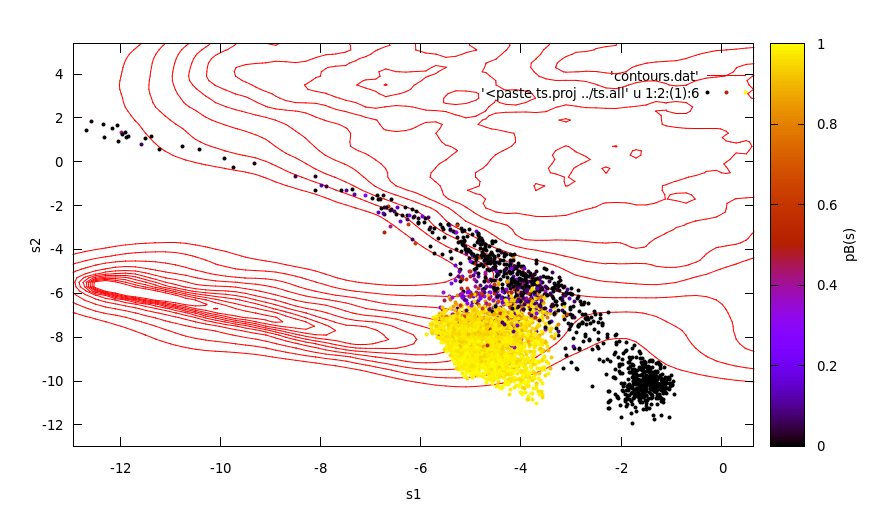
\includegraphics[width=0.5\textwidth]{figures/tsplot}
\end{figure}

\par\end{center}


\section{Analyzing the transition state ensemble}

We can then see how sketch-map coordinates work to describe high-energy
states and the transition state ensemble between the \emph{fcc }and
liquid-like states. You can find a file with the configurations saved
from the exercises in~\ref{sec:2d-committor}, or you can use one
from your own runs. You should first project the data points \begin{lstlisting}[language=matlabfloz][language=matlabfloz]
$ awk '{for (i=3; i<=NF; i++) printf "%s ", $i; print "" }' ts.all |
   dimproj -D 10 -d 2 -w -P lj38.lm -p lj38.ld -grid 15,16,151 
   -cgmin 3 -fun-hd 5,8,1 -fun-ld 5,2,2 > ts.proj 2> /dev/null
\end{lstlisting}And then do some gnuplot magic to overlay the sketch-map free energy
and the projection of the transition state data, colored according
to the committor.
\begin{lstlisting}[language=matlabfloz][language=matlabfloz]
gnuplot> set table 'contours.dat';
gnuplot> set view map; set contour; unset surface;
gnuplot> set cntrparam levels incremental 0.5,0.1,1.5; 
gnuplot> sp 'smap.fes' w l; unset table; res; set view map
gnuplot> sp 'contours.dat' w l, '<paste ts.proj ts.all' u 1:2:(1):6 w p lt pal pt 7 ps 0.5
\end{lstlisting}

The result should look similar to Fig.~\ref{fig:smap-tst}. Note
that the value of the committor is different from zero or one in the
region that is a saddle point on the sketch-map free energy -- although
a large portion of it is not sampled because the region we had selected
based on just $n_{6}$ and $n_{8}$ did not describe properly the
transition state ensemble. 


\section{Transferability of sketch-map}

{[}OPTIONAL{]} This far you have used a thorough sampling of the accessible
configuration space to build the initial map, and then projected additional
data samples onto this map. In most cases, however, one does not have
the luxury of complete sampling and so it is interesting to see how
sketch-map can ``fill in the blanks'' and give reasonable description
of the unexplored parts of the configurations space.

You can repeat the landmark selection and sketch-map construction
using as input only the data samples from the transition state ensemble,
and then project the whole trajectory from \texttt{out.all} onto this
partial map. Can you still recognize the most important features of
the energy landscape?

\bibliographystyle{ChemEurJ}
\bibliography{biblio}

\end{document}
